Como mencionado anteriormente, este trabalho tem como objetivo desenvolver o design de um circuito integrado para um DPD, partindo de um modelo previamente validado tanto em software quanto em hardware, especificamente em FPGA. O projeto foi dividido em quatro etapas principais:

\begin{itemize}
\item Estudo sobre PA e modelagem matemática;
\item Implementação em software do PA e do DPD;
\item Implementação do DPD em FPGA;
\item Design e validação do circuito implementado com a tecnologia de 8HP 130nm.
\end{itemize}


\section{Estudo sobre PA e modelagem matemática}
A etapa consistiu no estudo de modelagens de Amplificadores de potência para posteriormente fazer a modelagem do DPD, conforme apresentado no Capítulo \ref{chap:revi}, na qual foi feito todo o levantamento sobre os tipos de modelagem dos DPDs. O objetivo deste estudo é entender as diferentes abordagens de modelagem, avaliar seus desempenhos e identificar as mais adequadas para a aplicação em amplificadores de potência.

\section{Implementação em software} \label{sec:implsoft}

Nesta etapa, foi realizada a implementação do modelo DPD em software, utilizando a linguagem de programação Python. Esta linguagem amigável é amplamente difundida na comunidade acadêmica.

Para essa modelagem, foram coletados sinais de entrada e saída de um amplificador de potência classe AB, que utiliza um HEMT fabricado com tecnologia GaN. O amplificador foi excitado por um sinal portador de frequência de 900 MHz, modulado por um sinal de envelope WCDMA 3GPP com aproximadamente 3,84 MHz de largura de banda. Os dados de entrada e saída do amplificador de potência foram medidos usando um VSA Rohde \& Schwarz FSQ com uma taxa de amostragem de 61,44 MHz, conforme disponível em \cite{Bonfim2016}.

Em seguida, realizou-se o cálculo da estimativa do sinal utilizando números com vírgula fixa. Para verificar a precisão dessa estimativa em relação ao sinal original, calculou-se o NMSE. Para essa validação, os dados foram inicialmente divididos em conjuntos de extração e validação. A matriz de extração foi calculada com os dados de extração, utilizando o código disponível no anexo \ref{cod:mp}. Esse cálculo é essencial para a extração dos coeficientes do polinômio de memória. Após a extração dos coeficientes, calculou-se o modelo do PA, que foi então validado com os dados de validação. O NMSE obtido para um polinômio de $2^\circ$ grau com uma amostra memorizada foi de -23,57 dB.

Em seguida, o algoritmo foi ajustado para operar com números em vírgula fixa e o número total de bits foi reajustado para atingir a menor resolução possível, buscando o menor NMSE simulado, conforme ilustrado pelo anexo \ref{cod:mpint}. Por ser tratar de um cálculo em vírgula fixa, fez-se necessário uma readequação do resultado obtido entre cada multiplicação de forma a manter a resolução inicial.

\section{Implementação em FPGA}
Essa etapa envolve a implementação do DPD em FPGA, o que exige a paralelização das operações aritméticas. Em cada ciclo de clock, três operações são realizadas simultaneamente: o sinal atual é elevado ao quadrado, armazenado em um registrador de deslocamento dentro de uma matriz de extração \footnote{matriz que contém todas as potências e amostras anteriores necessárias para o cálculo da saída}, o cálculo do produto de todos os elementos da matriz de extração e a soma dos produtos entre os sinais do mesmo instante e seus respectivos coeficientes. Esse processo se repete \( P \) vezes, correspondendo ao grau \( P \) do polinômio de memória. Como consequência, a saída do DPD estará incompleta durante os primeiros \( P \) ciclos de clock, pois, nesse intervalo, o cálculo depende de amostras de sinais anteriores que ainda não foram processadas, resultando em uma saída parcial.
 A Figura \ref{fig:diagramaprocess} ilustra como esse processo está dividido entre cada ciclo de clock.
 
\begin{figure}[htbp!]
  \centering
  \captionsetup{justification=centering}
  \caption*{Fonte: Autor}
  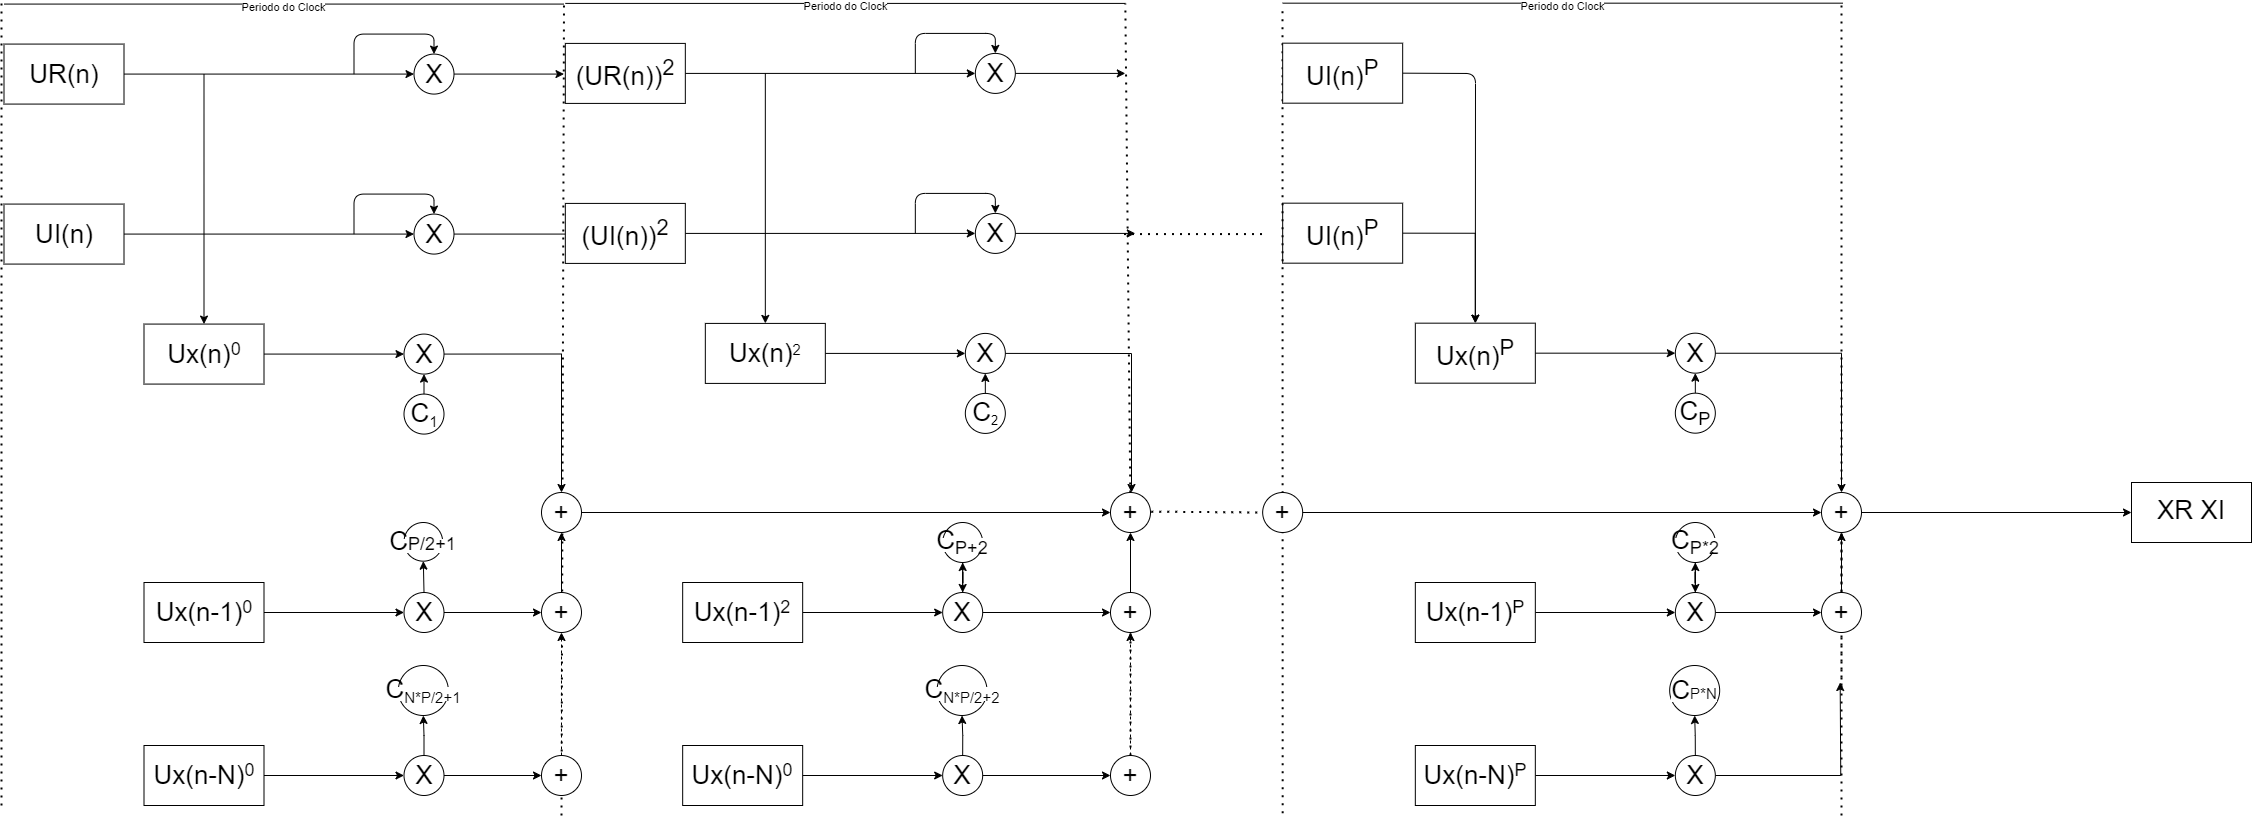
\includegraphics[width=0.80\textwidth]{diagrama_process.png}
  \caption{Processo de cálculo da saída}
  \label{fig:diagramaprocess}
\end{figure}
Conforme exibido no diagrama, cada etapa do processo fornece os dados necessários para a próxima fase do cálculo com um atraso de um ciclo de clock. Contudo, é importante destacar que o processo completo demanda ciclos adicionais, uma vez que o sinal de saída só é registrado na borda de subida seguinte do clock, garantindo a sincronização adequada no fluxo de dados.

\subsection{Design e Validação do Circuito Lógico}  
O design da síntese lógica do circuito DPD foi realizado seguindo o fluxo VLSI, utilizando a tecnologia BiCMOS 130 nm 8HP. O processo abrangeu desde a descrição em alto nível até a validação final do circuito.  

Inicialmente, a descrição em VHDL foi estruturada com base em um modelo comportamental que prioriza a eficiência computacional e a paralelização das operações. Essa abordagem assegura que o design inicial seja compatível com as restrições impostas pelas etapas subsequentes de síntese e layout.  

A síntese lógica foi conduzida na ferramenta Cadence Genus, utilizando células padrão otimizadas para a tecnologia alvo. Durante essa etapa, foram exploradas configurações alternativas de pipeline e estratégias de paralelização para minimizar atrasos críticos e melhorar a taxa de transferência.  

Além disso, relatórios detalhados contendo informações sobre área ocupada, consumo de energia e número de células lógicas utilizadas foram gerados ao final da síntese lógica. Esses relatórios serviram como base para avaliar a eficiência do circuito e orientar ajustes nas etapas subsequentes, garantindo que o design final atendesse às especificações do projeto de forma otimizada.

Após a síntese, os arquivos Verilog e SDF gerados foram analisados em simulações pós-síntese com a ferramenta Cadence NCLaunch. A principal preocupação foi verificar o impacto do atraso nas operações críticas do DPD, validando o funcionamento lógico sob as condições especificadas de temporização.  

%Na etapa de PAR (\textit{place and route}), a ferramenta **Cadence Innovus** foi utilizada para posicionar as células e roteá-las, considerando as propriedades físicas do processo BiCMOS 130 nm. Durante essa etapa, foi necessário ajustar a densidade do layout para reduzir capacitâncias parasitas e otimizar as linhas de interconexão mais longas, especialmente nas áreas onde ocorre maior comunicação entre os blocos do circuito.  

%O circuito passou por simulações pós-layout para avaliação do impacto de parasitas no desempenho geral. Nesse ponto, utilizou-se o modelo extraído com informações de resistência e capacitância gerado pelo Innovus, combinado com os atrasos descritos no arquivo SDF. Essas simulações foram fundamentais para ajustar os elementos críticos e garantir que o circuito atenda às especificações de frequência de operação e robustez em relação a variações de processo e temperatura.  

%Por fim, os resultados das simulações pós-síntese e pós-layout foram comparados com as simulações comportamentais para verificar a consistência funcional. O circuito validado foi exportado para os arquivos GDSII, que representam a geometria final do layout pronta para fabricação.  

